\chapter{随机变量及其分布}
\section{随机变量}
\dfn{随机变量}{
    设随机试验的样本空间为$S$,称定义在$S$上的实值单值函数$X=X(\omega)$为\vocab{随机变量}.\\
    亦即
    \[X:\omega\mapsto x_i \in \RR\,\, \mathrm{i.e.}\,\,S\rightarrow\RR\]
}
实际上,$\Pr(X=a)$是$A=\{\omega|X(\omega)=a\}$的简记.
\section{离散型随机变量及其分布}
设$X$是一个随机变量,如果$X$的所有可能取值为有限个或可列无限多个,则称$X$为\vocab{离散型随机变量}.
\dfn{离散型随机变量分布律}{
    设$X$是一个离散型随机变量,如果
    \[\Pr(X=x_k)=p_k,k=1,2,\cdots\]
    则称$p_k$为$X$的\vocab{分布律}或\vocab{概率分布},亦称\vocab{概率质量函数}(PMF). 记为$f_X(x)$.
}
就是高中所学之分布列.
\subsection{常用离散分布}
\subsubsection{两点分布}
\dfn{两点分布}{
    设$X$的分布律为
    \[\Pr(X=k)=\begin{cases}
            p,   & k=x_1 \\
            1-p, & k=x_2
        \end{cases}\]
    其中$0<p<1$,则称$X$服从以$p$为参数的\vocab{两点分布}.
}
若$X$服从$x_1 = 1,x_2 = 0$处参数为$p$的两点分布,则称其服从参数为$p$的\vocab{0-1分布}.
\subsubsection{二项分布}
\leftnote[1cm]{当$n=1$时,二项分布退化为0-1分布.}
\dfn{二项分布}{
    设$X$的分布律为
    \[\Pr(X=k)=\binom{n}{k}p^k(1-p)^{n-k},\,\,k=0,1,\cdots,n\]
    其中$n$为正整数,$0<p<1$,则称$X$服从参数为$n,p$的\vocab{二项分布},记为$X\sim B(n,p)$.
}
\leftnote{$\sim$记号就是\textbf{服从}的意思}
二项概率总存在一个最大值$M$ s.t. \((n+1)p-1\leq M<(n+1)p\).
\subsubsection{Poisson分布}
\dfn{Poisson分布}{
设$X$的分布律为
\[\Pr(X=k)=\frac{\lambda^k}{k!}e^{-\lambda},\,\,k=0,1,\cdots\]
其中$\lambda>0$,则称$X$服从参数为$\lambda$的\vocab{Poisson分布},记为$X\sim P(\lambda)$.
}
因为$e^x=1+\sum_{n=1}^{\infty}\frac{x^n}{n!}$,将$x$换为$\lambda$可得泊松分布的概率和为1.
\section{累积分布函数}
\subsection{随机变量的分布函数}
\dfn{随机变量CDF}{
    设$X$是一个随机变量,对任意实数$x$,定义
    \[F(x)=\Pr(X\leq x)\in [0,1]\]
    称$F(x)$为$X$的\vocab{累积分布函数}(CDF). 有时记作$F_X(x)$或$X\sim F(x)$.
}
分布函数$F(x)$的值就表示$X$落在区间$(-\infty,x]$的概率.
\subsubsection{性质}
\begin{enumerate}
    \item \textit{单调非减性}: $x_1<x_2\Rightarrow F(x_1)\leq F(x_2)$
    \item $F(-\infty) = \lim_{x\rightarrow -\infty}F(x) = 0,\,\,F(+\infty) = \lim_{x\rightarrow +\infty}F(x) = 1$.
    \item \textit{右连续性}: $\lim_{x\rightarrow x_0^+}F(x) = F(x_0)$
\end{enumerate}
具有上述性质的函数一定是某个随机变量的CDF.
\clearpage
\subsection{离散型随机变量的分布函数}
在上述基础上,对于离散型随机变量$X$有CDF:
\[F(x) = \Pr(X\leq X) = \sum_{x_i\leq x}\Pr(X=x_i)\]

\begin{figure}[h]
    \centering
    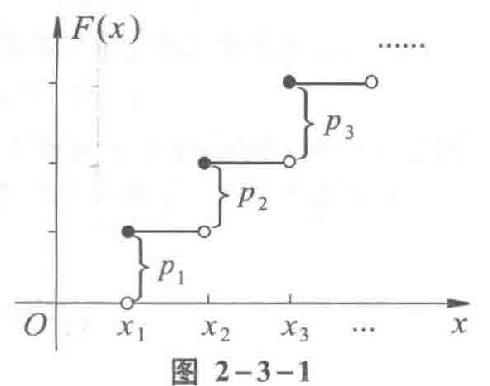
\includegraphics[scale=.5]{cdf_discrete}
    \caption{阶梯型CDF}
\end{figure}
$F(x)$是一个\vocab{阶梯型函数},在点$x_i$处的跃度为$\Pr(X=x)$.
可以看出阶梯型函数符合CDF之性质:总是右连续的;而作为一个分段函数来说,其各段区间总是左闭右开的.
\nt{
    考题中由CDF反推分布列可以根据每一个左侧端点得到对应的随机变量$x_i$.\\
    计算分布列时,有公式$\Pr{a\leq X< b} = F(b) - F(a)$.
}
随机变量$X$的CDF为阶梯型函数$\Leftrightarrow$ $X$是离散型随机变量.